\documentclass[12pt,letterpaper,titlepage,en-US]{article}

\usepackage{basicstyle}
\usepackage{report}
\usepackage{knit}

%
% Homework Details
%   - Title
%   - Due date
%   - Class
%   - Section/Time
%   - Instructor
%   - Author
%

\newcommand{\hmwkTitle}{Mini Project \#3}
\DTMsavetimestamp{DueDate}{2017-03-07T16:00:00-06:00}
\newcommand{\hmwkClass}{CS 6313.001}
\newcommand{\hmwkClassName}{Statistical Methods for Data Science}
\newcommand{\hmwkClassInstructor}{Instructor: Pankaj Choudhary}
\newcommand{\hmwkAuthorName}{Hanlin He / Lizhong Zhang}
\newcommand{\hmwkAuthorNetID}{hxh160630 / lxz160730}

\newcommand{\hmwkAuthorOneName}{Lizhong Zhang (lxz160730)}
\newcommand{\hmwkAuthorTwoName}{Hanlin He (hxh160630)}



%
% Title Page
%

\title{
    \vspace{1in}
    \textmd{\textbf{\hmwkClassName \\\hmwkClass:\ \hmwkTitle }}\\
    \normalsize\vspace{0.1in}\small{Due\ on\ \DTMusedate{DueDate}\ at \DTMusetime{DueDate} }\\
    \vspace{0.1in}\large{\textit{\hmwkClassInstructor}}\\
    \vspace{0.5in}
\includegraphics[height=2.4em]{UTD_logo_BW}\\
    \vspace{2in}
}

\author{\textbf{\hmwkAuthorName\ \footnotesize{(\hmwkAuthorNetID)}} \\ }
\date{}
\makeindex

\begin{document}
\maketitle

% \pagenumbering{Roman}

% \tableofcontents

% \pagebreak
\pagenumbering{arabic}


\section*{Contribution}
Both team members made the same contribution in this project.

\section{Answers}
\subsection{Blood Pressure Measurement}
\subsubsection{Boxplots}
The boxplots are shown in \cref{pic1}:
\begin{figure}[H]
\caption{Boxplots}
\label{pic1}
\centering
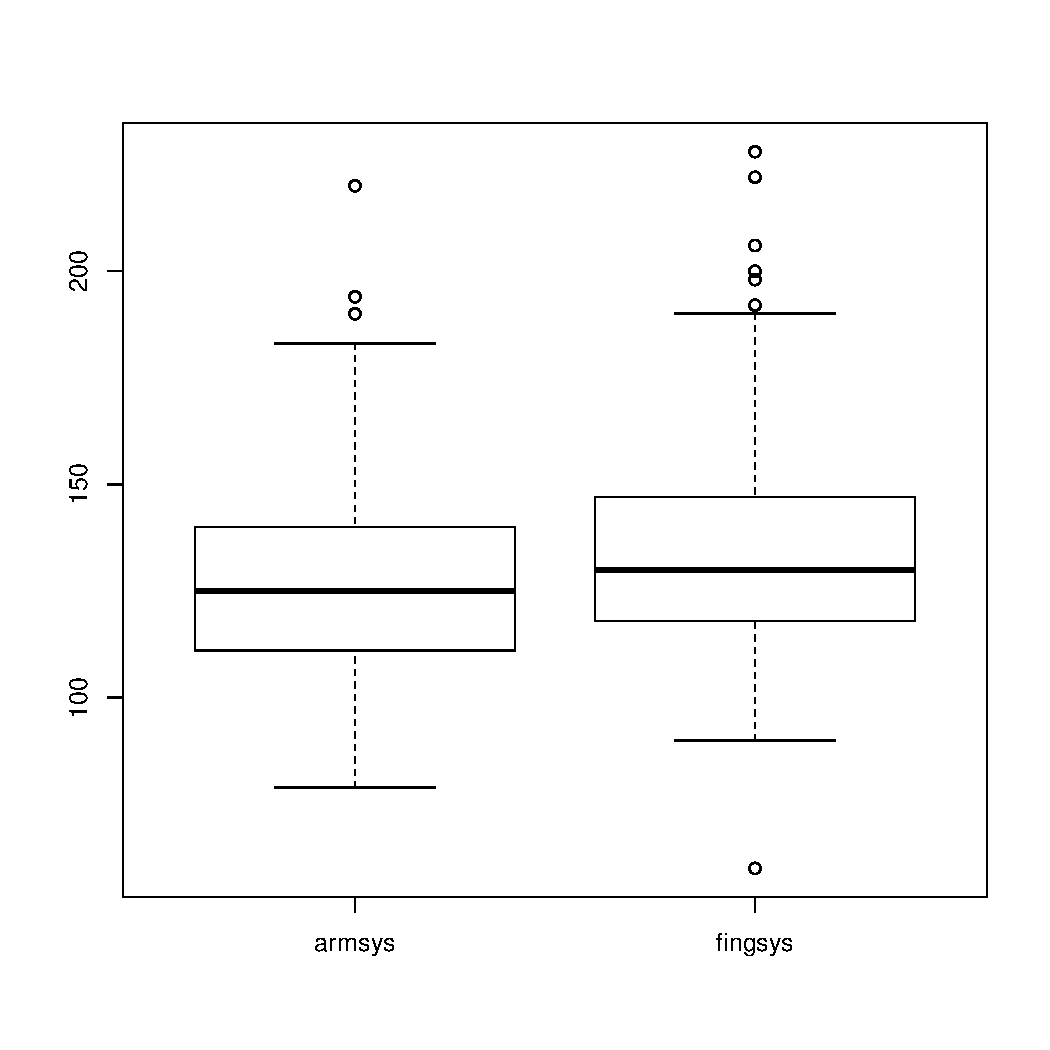
\includegraphics[width=.6\textwidth]{figure/pic1.pdf}
\end{figure}
From my point of view, we could see that based on boxplots, two distributions are not similar. The data in Finger method is slightly larger than the data in Arm method, and Finger method is slightly right-skewed.

\pagebreak
\subsubsection{Histograms \& QQplot}

The histograms are shown in \cref{pic2}:
\begin{figure}[H]
\caption{Histogram}
\label{pic2}
\centering
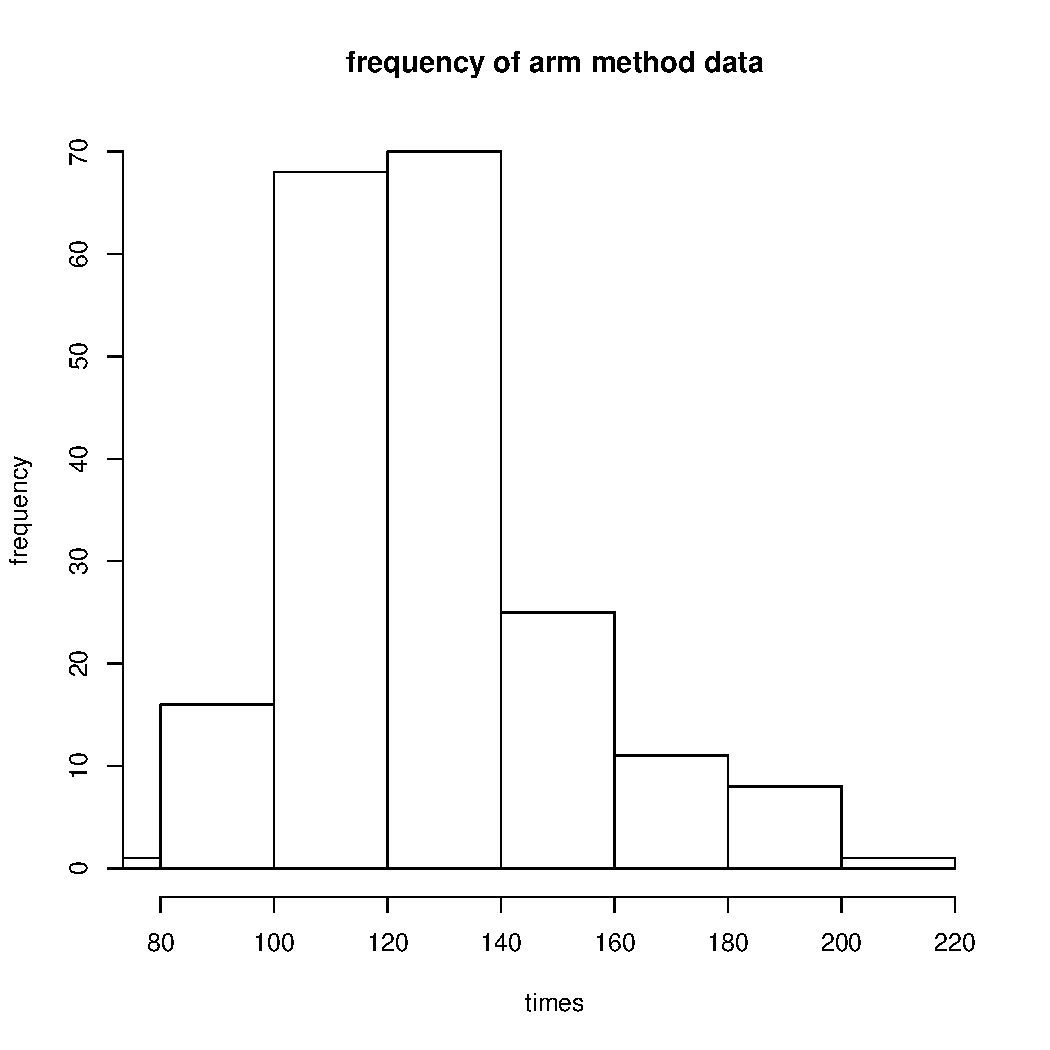
\includegraphics[width=.49\textwidth]{figure/pic2.pdf}
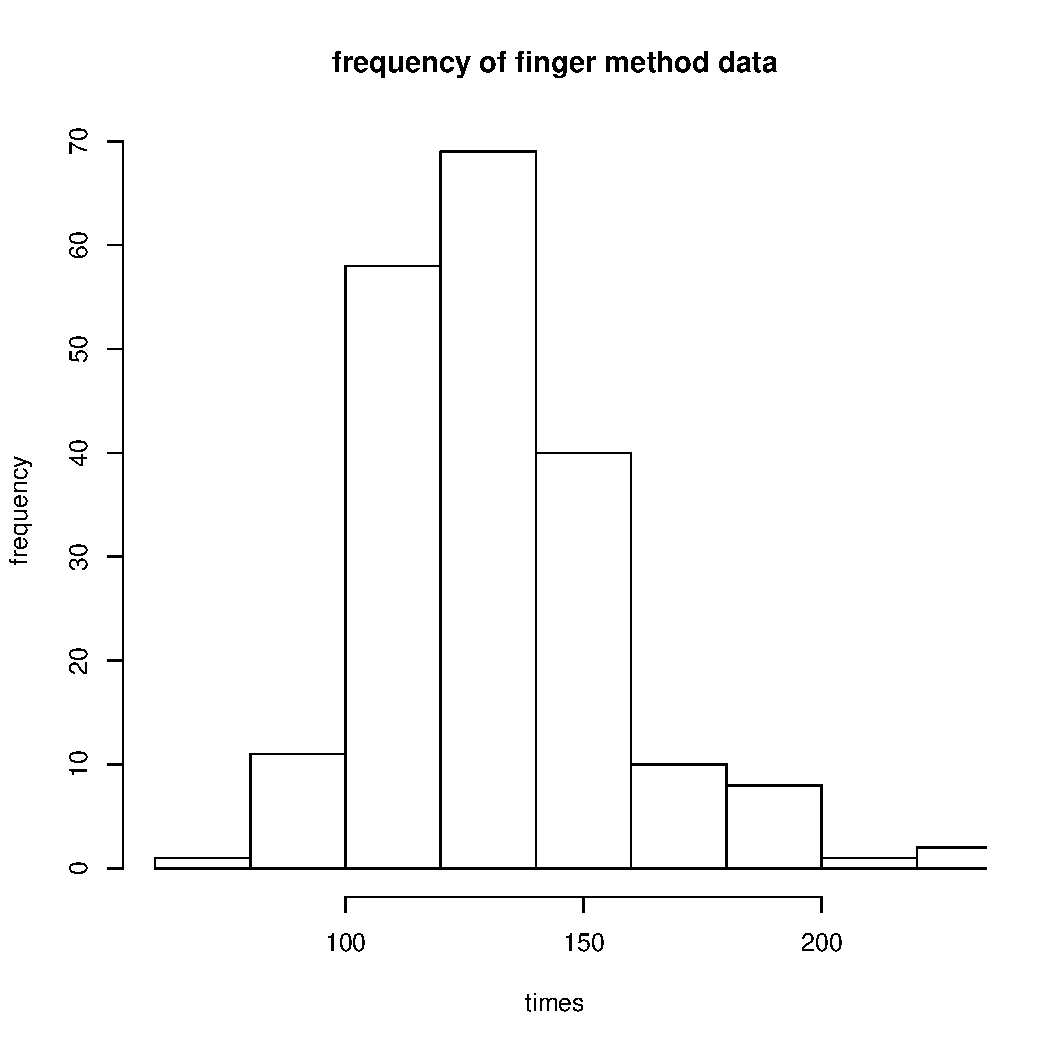
\includegraphics[width=.49\textwidth]{figure/pic3.pdf}
\end{figure}

The QQplots are shown in \cref{pic4}:
\begin{figure}[H]
\caption{QQplot}
\label{pic4}
\centering
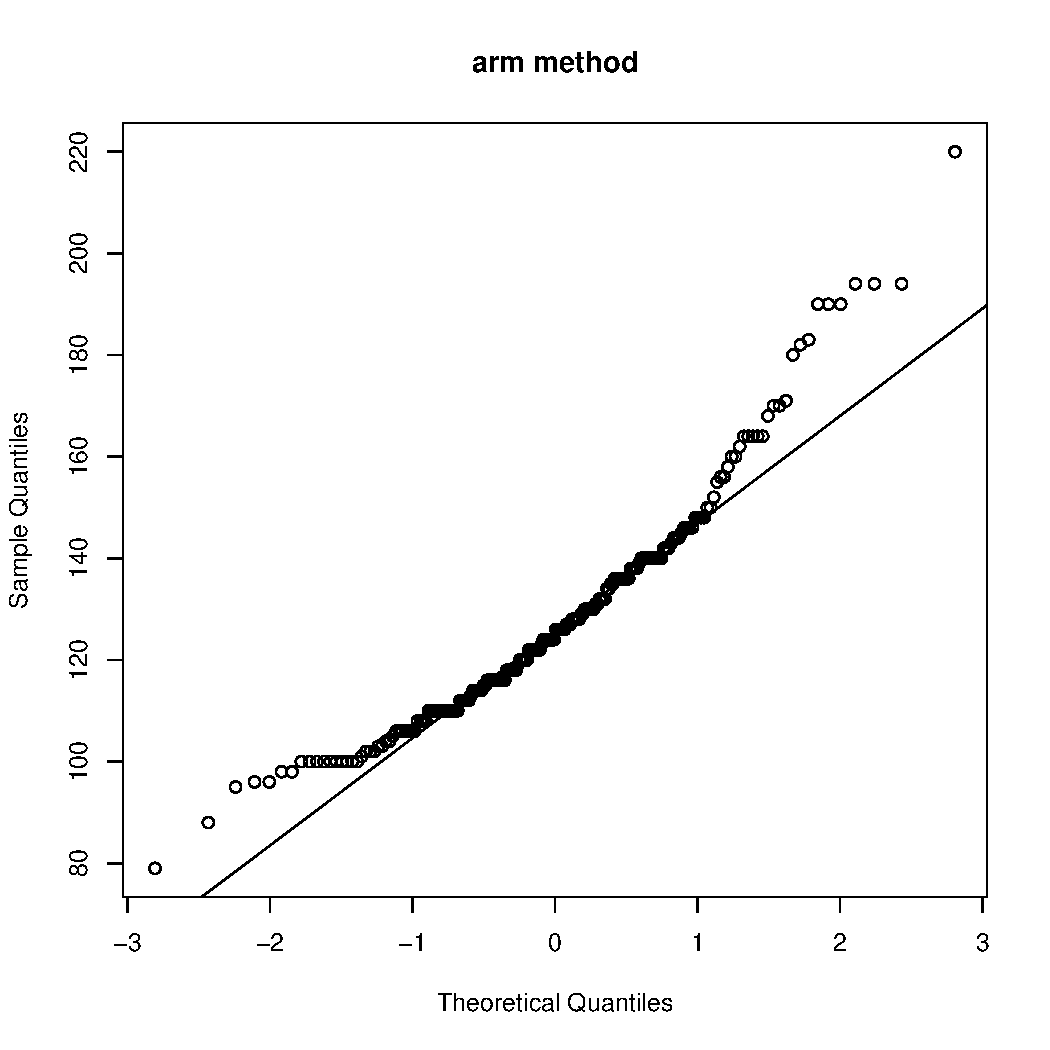
\includegraphics[width=.49\textwidth]{figure/pic4.pdf}
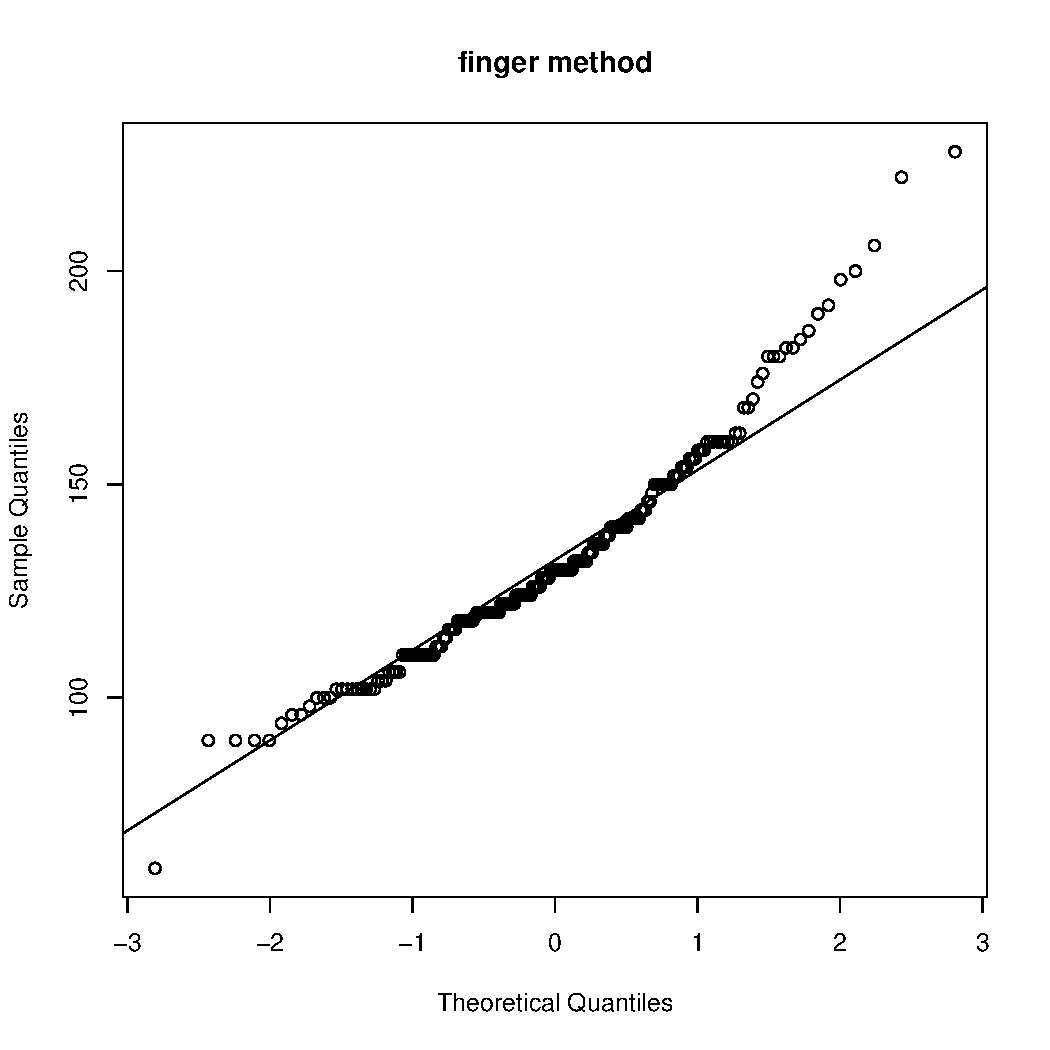
\includegraphics[width=.49\textwidth]{figure/pic5.pdf}
\end{figure}

Based on histograms and QQplots, we could see that the assumptions of normality are not reasonable.

In histograms, we could see that both distributions are slightly right-skewed.
And in QQplots, both distributions have many outliers.

\subsubsection{CI}

The CI is $[-0.5208386, 9.1108386]$.

According above result, we can conclude that the two methods have identical means.
But this is a borderline case. We need more data for a more precise conclusion.


\subsection{}

CI for the same sample size $n$ of different $p$ is shown in \cref{sndp}
\begin{figure}[H]
    \caption{Confidence Intervals for $n = 50$ and Different $p$}
    \label{sndp}
    \centering
    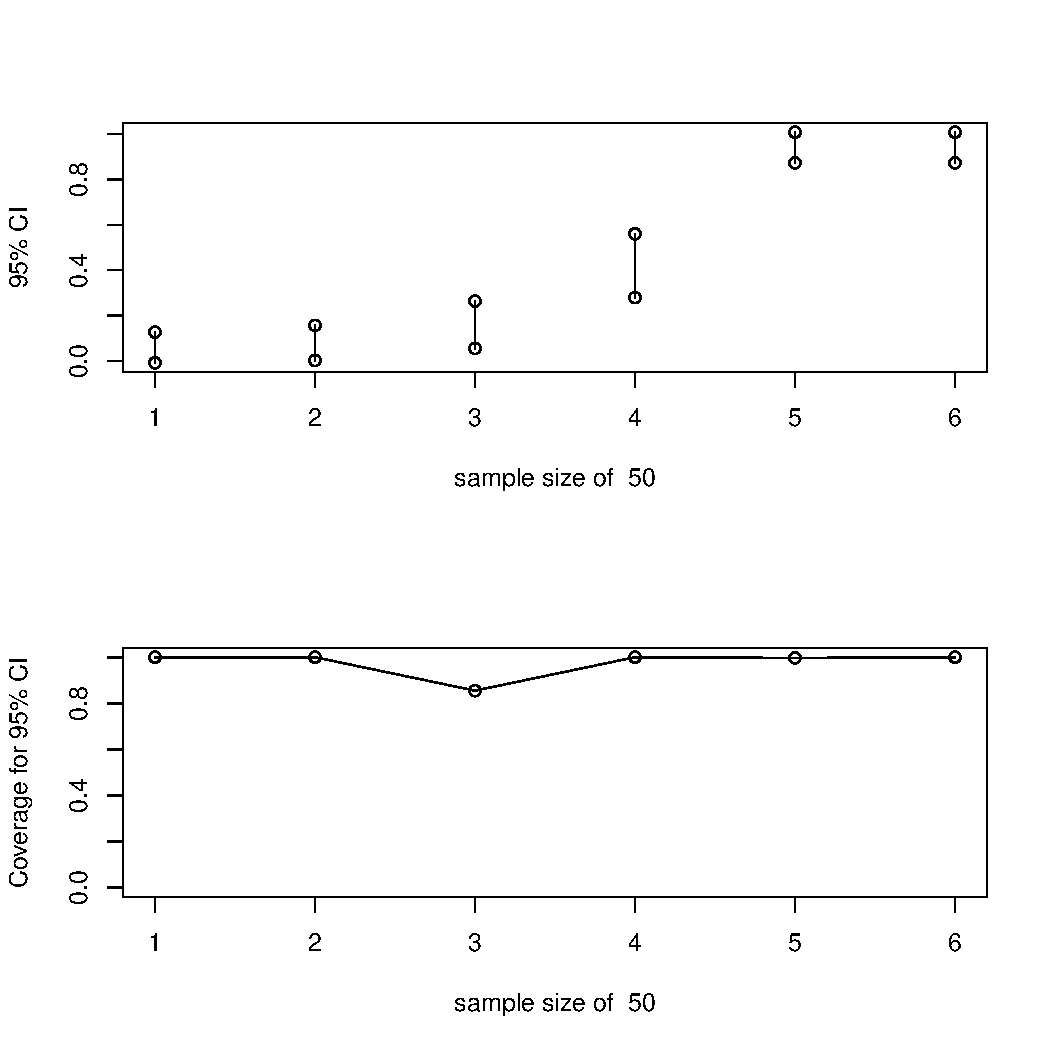
\includegraphics[width=.9\textwidth]{figure/sameN50.pdf}
\end{figure}
\begin{figure}[H]
    \caption{Confidence Intervals for Same $n = 100$ and Different $p$}
    \label{sndp}
    \centering
    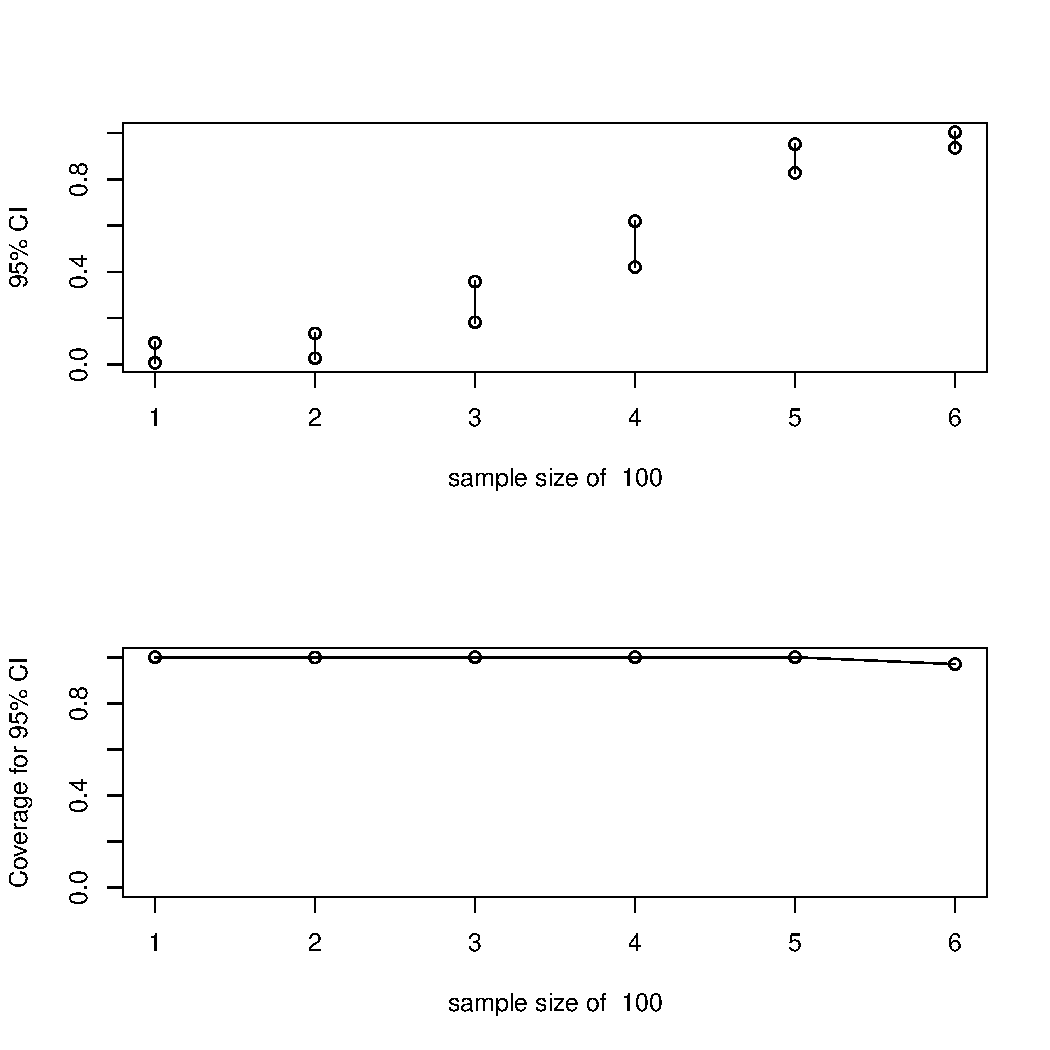
\includegraphics[width=.9\textwidth]{figure/sameN100.pdf}
\end{figure}
\begin{figure}[H]
    \caption{Confidence Intervals for Same $n = 300$ and Different $p$}
    \label{sndp}
    \centering

    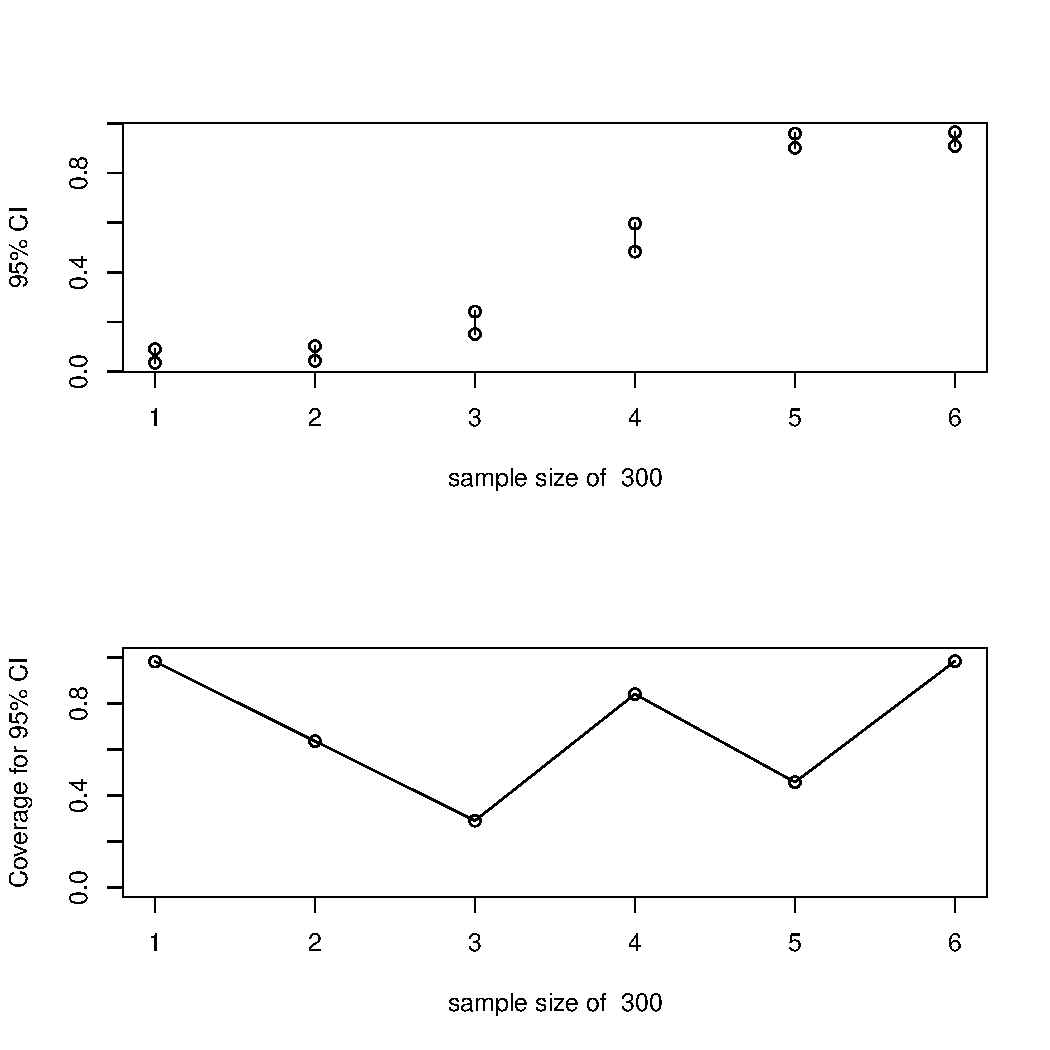
\includegraphics[width=.9\textwidth]{figure/sameN300.pdf}
\end{figure}
\begin{figure}[H]
    \caption{Confidence Intervals for Same $n = 500$ and Different $p$}
    \label{sndp}
    \centering

    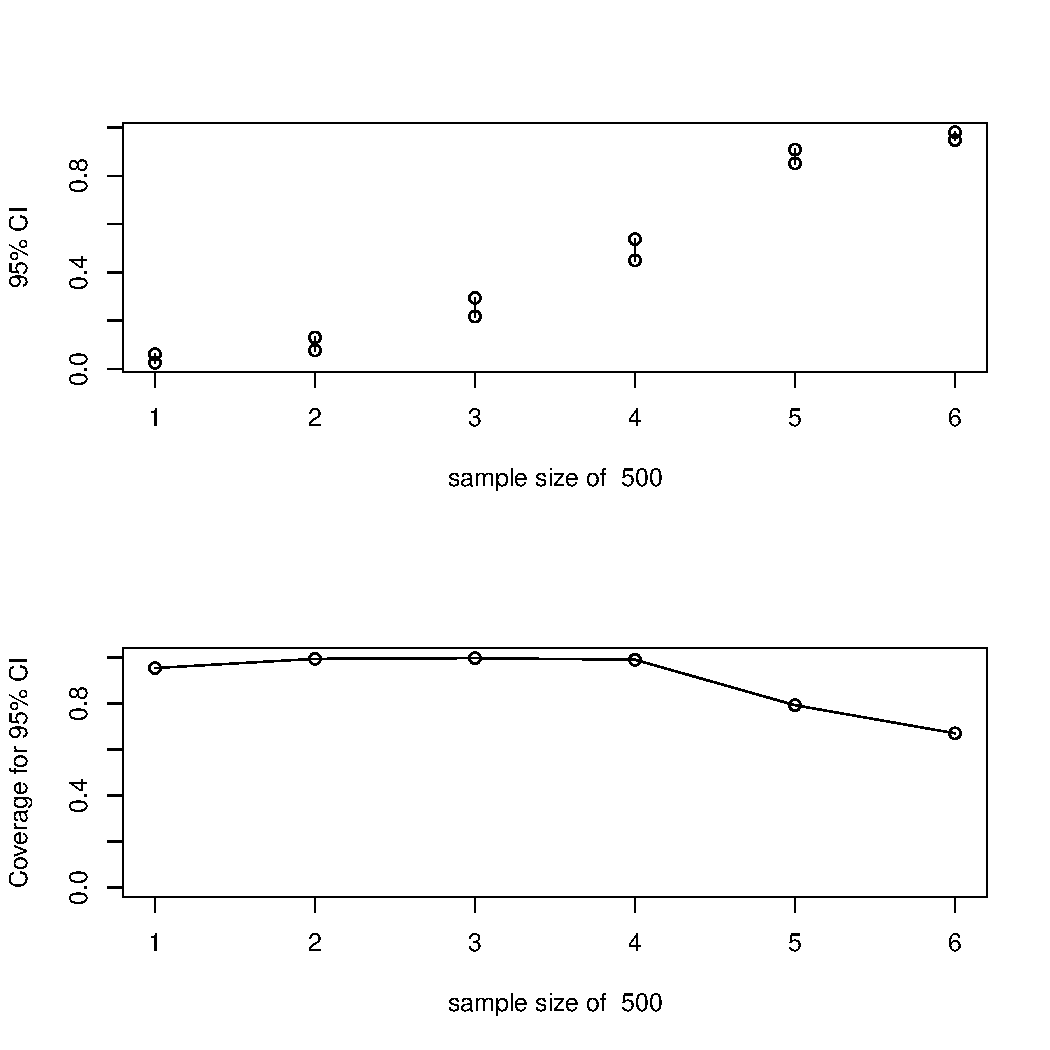
\includegraphics[width=.9\textwidth]{figure/sameN500.pdf}
\end{figure}
\begin{figure}[H]
    \caption{Confidence Intervals for Same $n = 1000$ and Different $p$}
    \label{sndp}
    \centering

    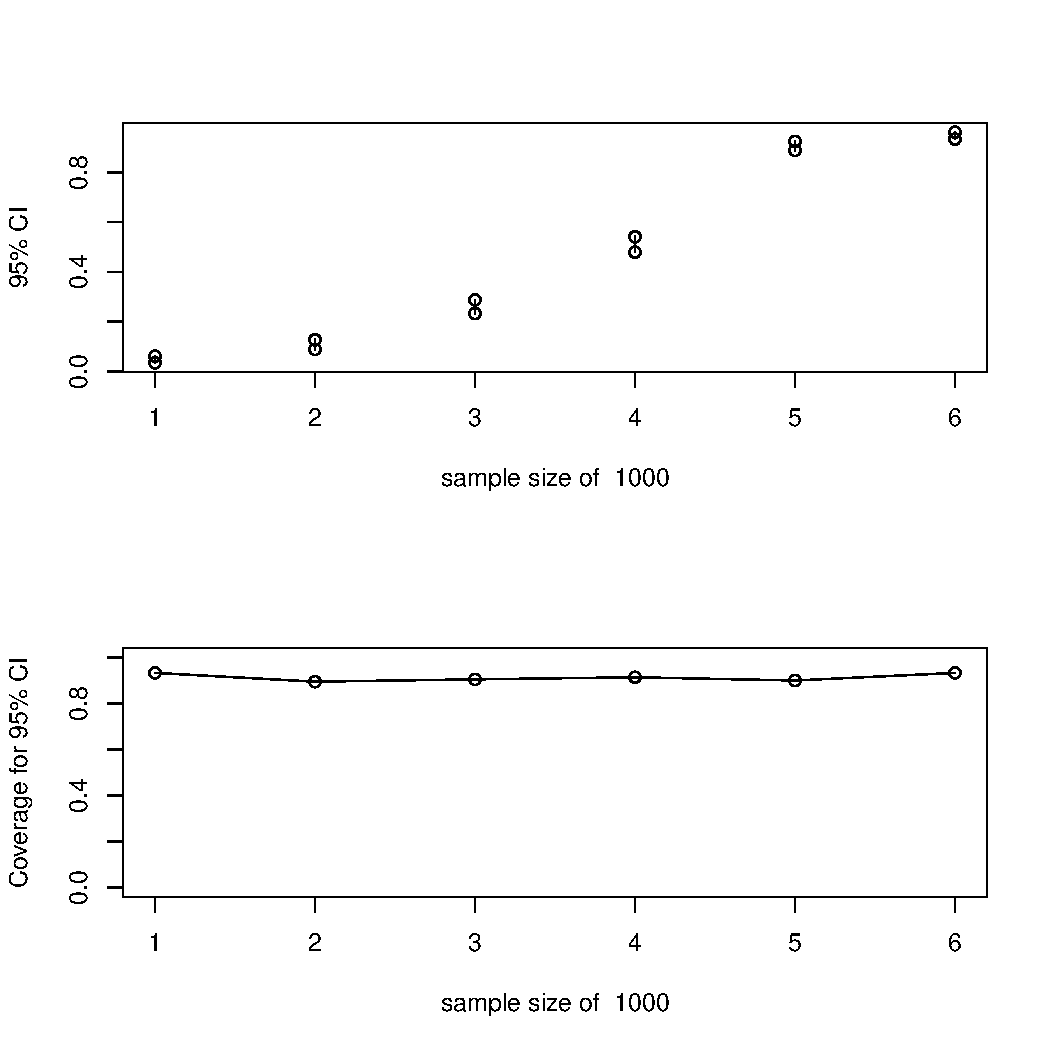
\includegraphics[width=.9\textwidth]{figure/sameN1000.pdf}

\end{figure}


CI for the same $p$ with different sample size $n$ is shown in \cref{spdn}
\begin{figure}[H]
    \caption{Confidence Intervals for $p = 0.05$ and Different $n$}
    \label{spdn}
    \centering
    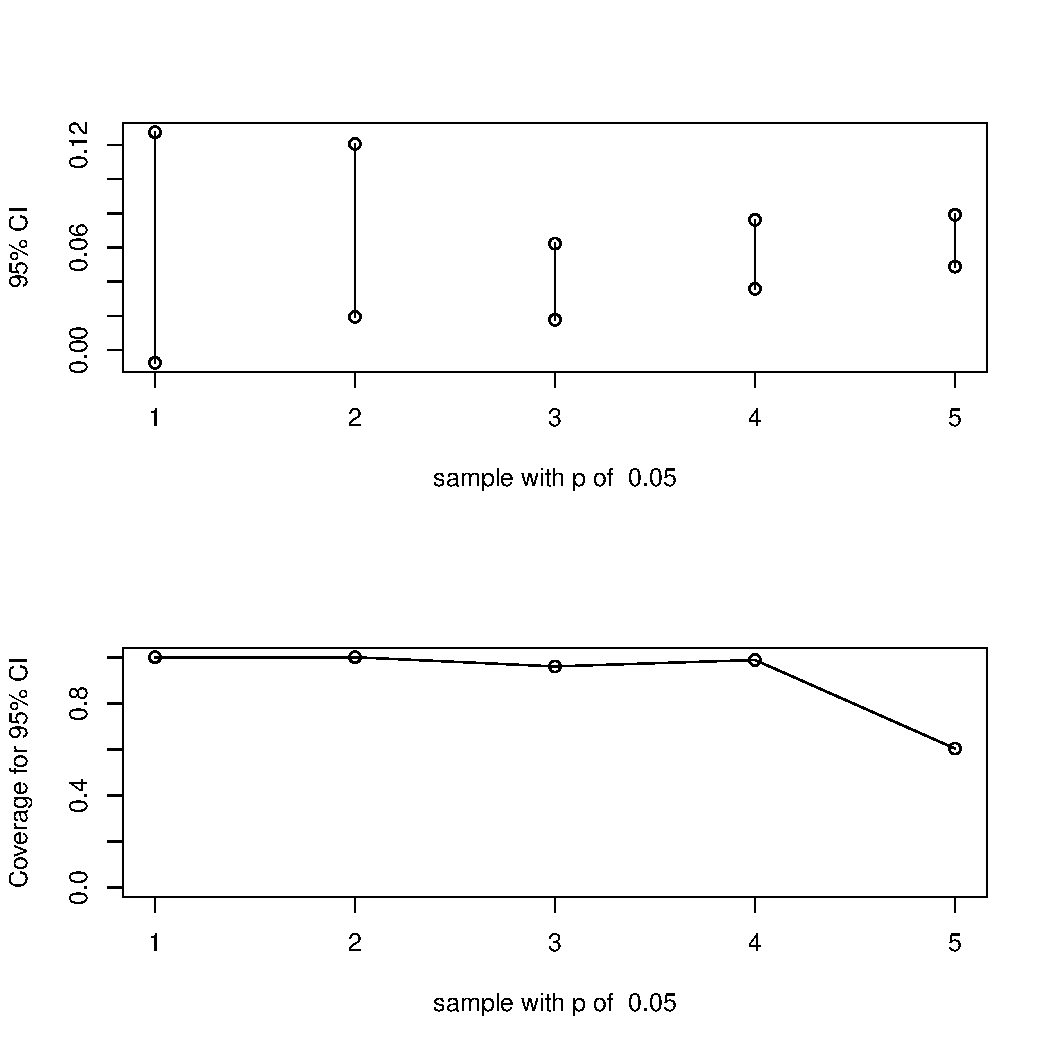
\includegraphics[width=.9\textwidth]{figure/sameP005.pdf}
\end{figure}
\begin{figure}[H]
    \caption{Confidence Intervals for $p = 0.1$ and Different $n$}
    \label{sndp}
    \centering
    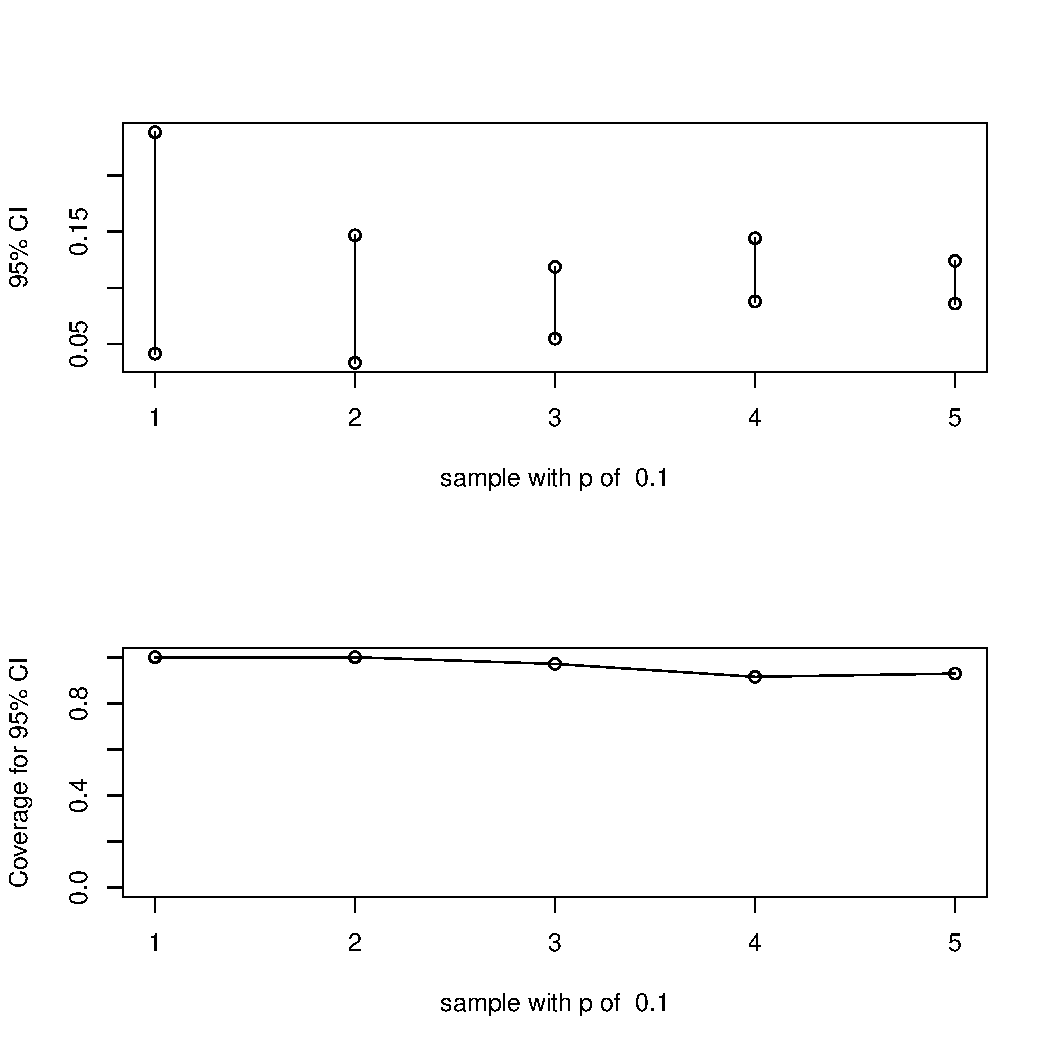
\includegraphics[width=.9\textwidth]{figure/sameP01.pdf}
\end{figure}
\begin{figure}[H]
    \caption{Confidence Intervals for $p = 0.25$ and Different $n$}
    \label{sndp}
    \centering
    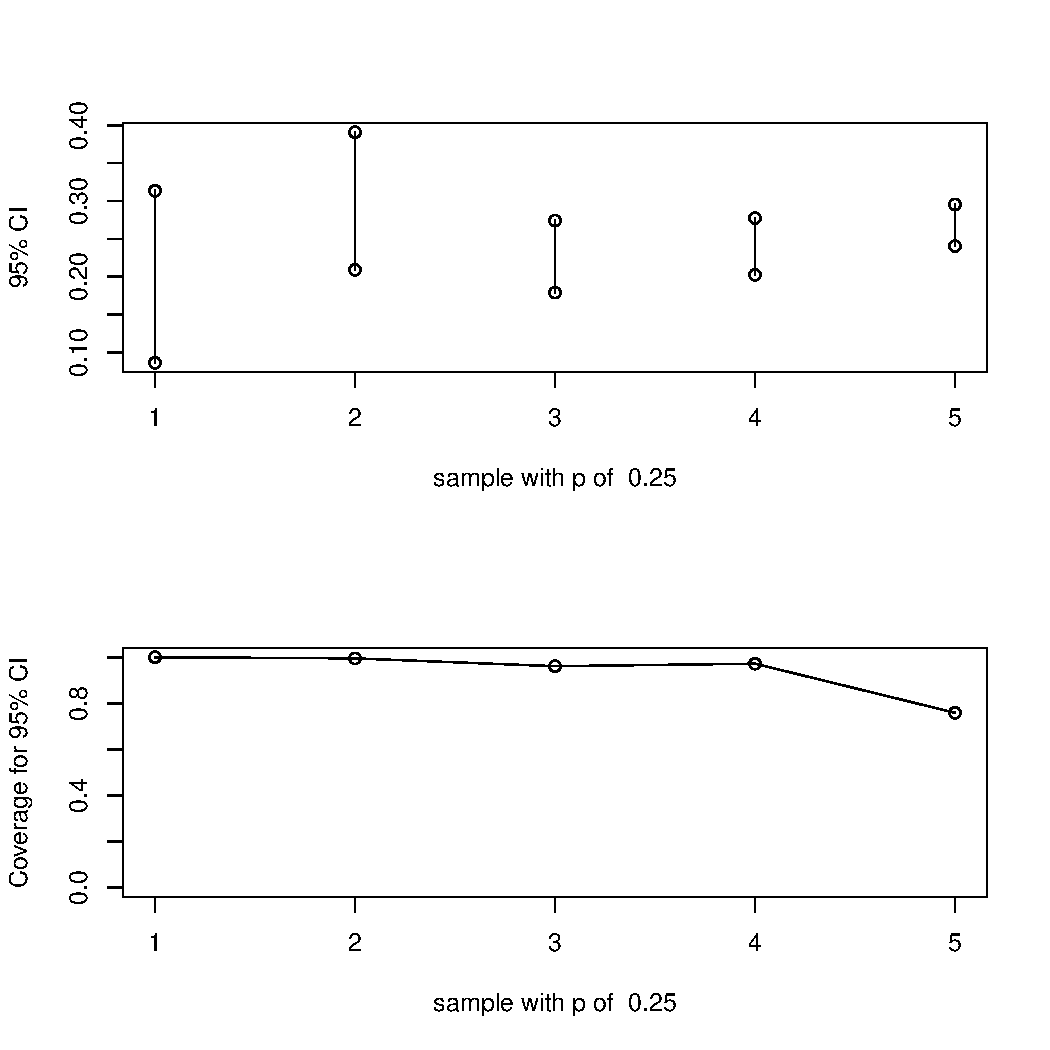
\includegraphics[width=.9\textwidth]{figure/sameP025.pdf}
\end{figure}
\begin{figure}[H]
    \caption{Confidence Intervals for $p = 0.5$ and Different $n$}
    \label{sndp}
    \centering
    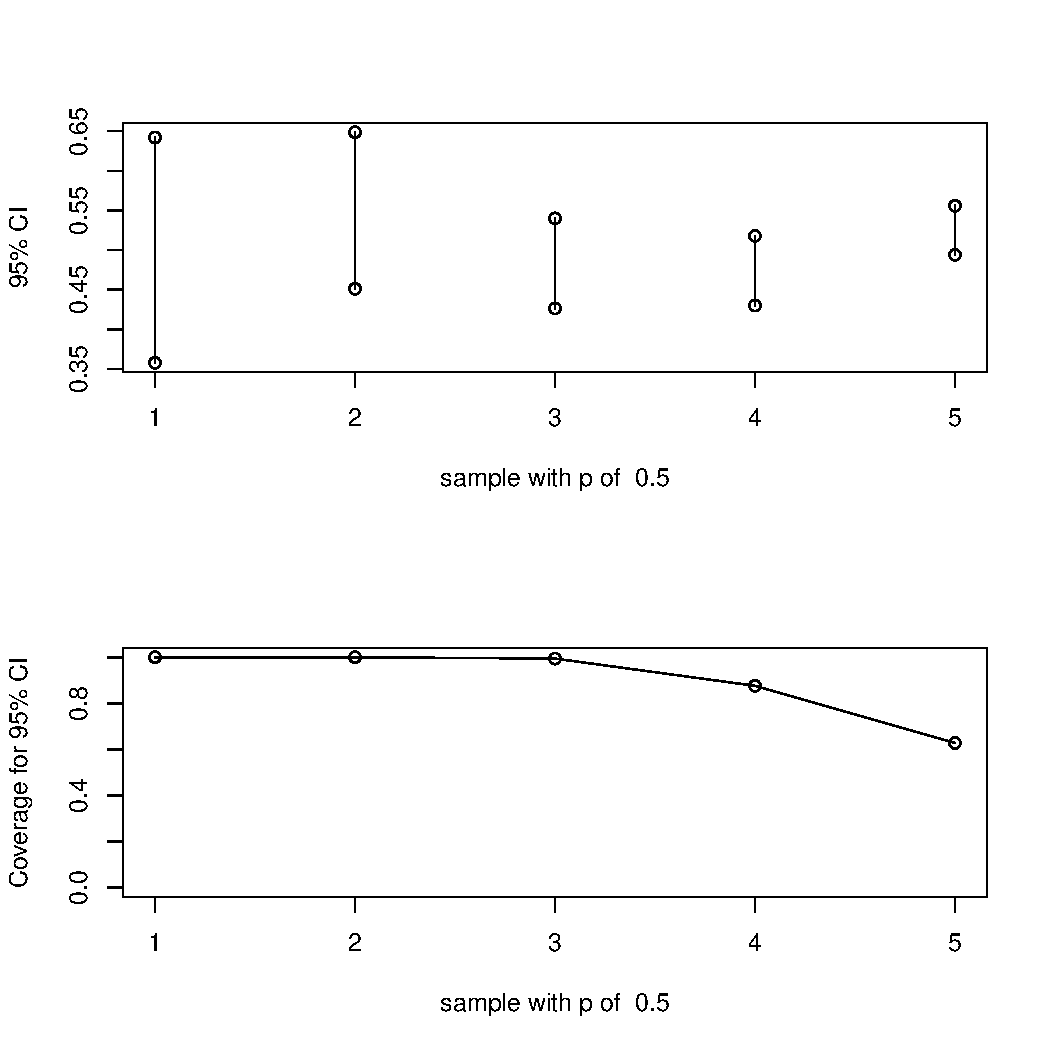
\includegraphics[width=.9\textwidth]{figure/sameP05.pdf}
\end{figure}
\begin{figure}[H]
    \caption{Confidence Intervals for $p = 0.9$ and Different $n$}
    \label{sndp}
    \centering
    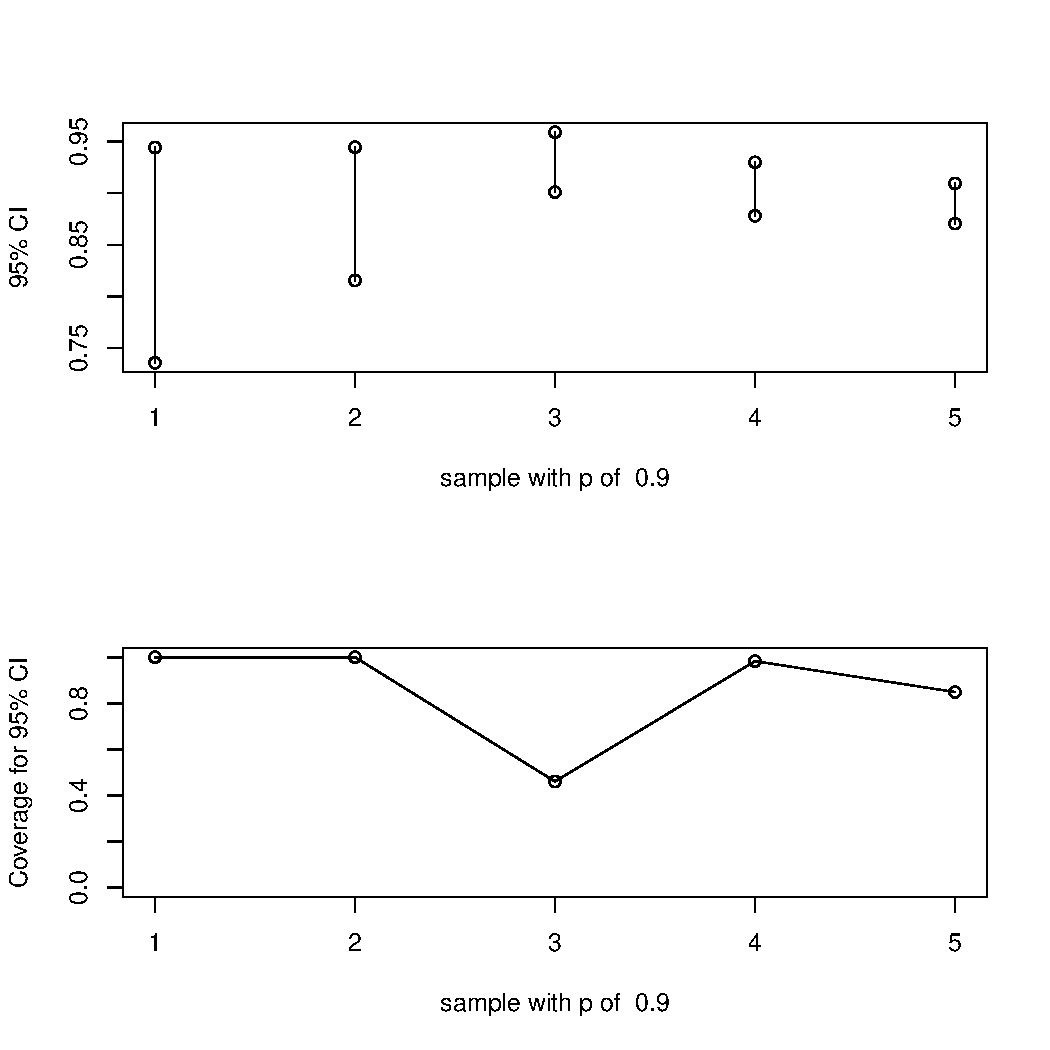
\includegraphics[width=.9\textwidth]{figure/sameP09.pdf}
\end{figure}
\begin{figure}[H]
    \caption{Confidence Intervals for $p = 0.95$ and Different $n$}
    \label{sndp}
    \centering
    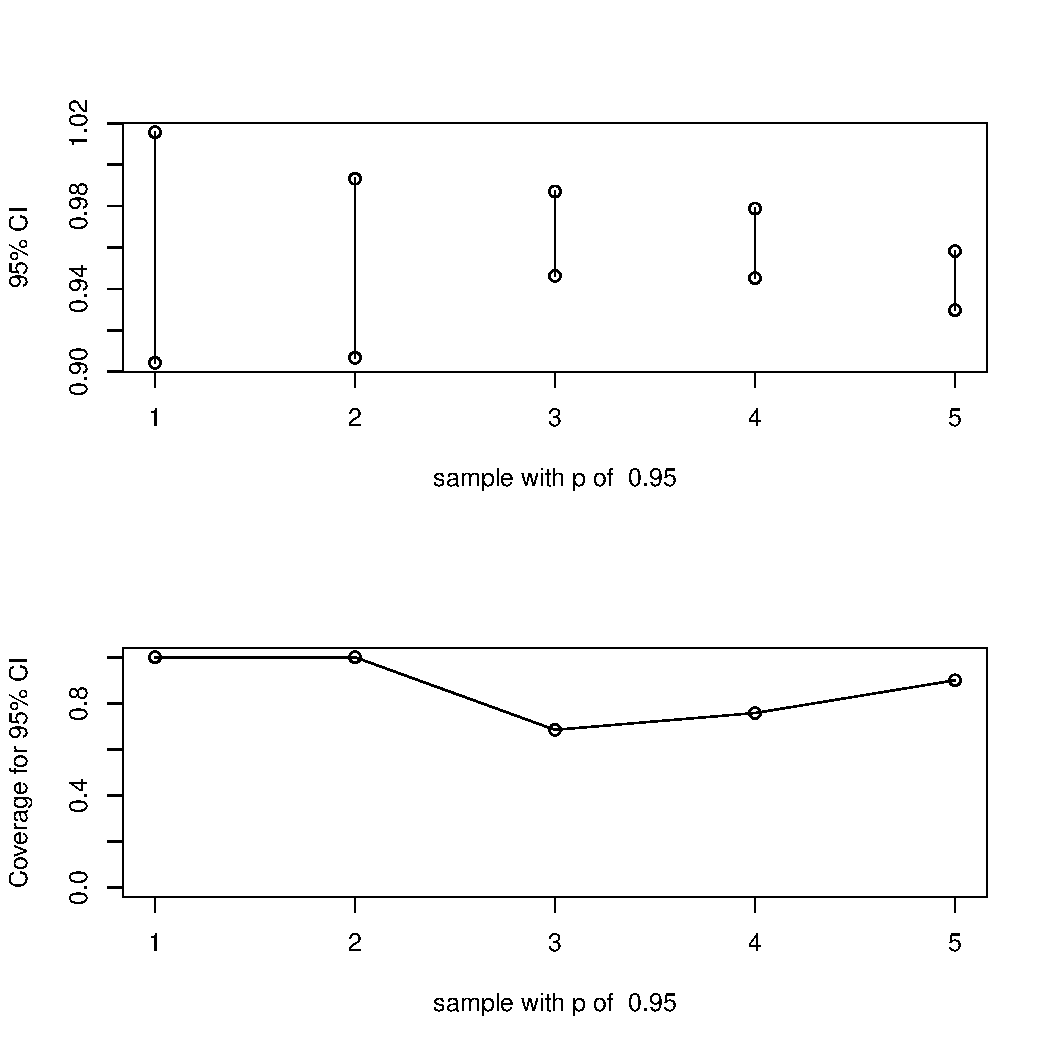
\includegraphics[width=.9\textwidth]{figure/sameP095.pdf}
\end{figure}


Based on the output tables and confidence interval, we know that with the increase of $n$, the accuracy of confidence interval for a population proportion will be higher for same $p$. On the other hand, for same $n$, when $p = 0.5$, the CI is largest in general.

For this problem, $n = 100$ is recommended, and the answer does not rely on $p$.

\pagebreak

\section{R Code}


\begin{knitrout}
\definecolor{shadecolor}{rgb}{0.969, 0.969, 0.969}\color{fgcolor}\begin{kframe}
\begin{alltt}
\hlcom{# Read data from file.}
\hlstd{prostatecancer} \hlkwb{<-} \hlkwd{read.table}\hlstd{(}\hlkwc{file}\hlstd{=}\hlstr{"prostate_cancer.csv"}\hlstd{,} \hlkwc{sep}\hlstd{=}\hlstr{","}\hlstd{,} \hlkwc{header}\hlstd{=T)}

\hlcom{# Create fig folder to store plot.}
\hlkwa{if}\hlstd{(}\hlopt{!}\hlkwd{dir.exists}\hlstd{(}\hlstr{"fig"}\hlstd{))} \hlkwd{dir.create}\hlstd{(}\hlstr{"fig"}\hlstd{)}

\hlcom{# Attach data to memory.}
\hlkwd{attach}\hlstd{(prostatecancer)}
\hlstd{psalog} \hlkwb{<-} \hlkwd{log}\hlstd{(psa)}

\hlcom{# Box plot for psa.}
\hlkwd{pdf}\hlstd{(}\hlstr{"fig/boxplotpsa.pdf"}\hlstd{,} \hlkwc{width}\hlstd{=}\hlnum{7}\hlstd{,} \hlkwc{height}\hlstd{=}\hlnum{7}\hlstd{)}
\hlkwd{boxplot}\hlstd{(psa)}
\hlkwd{dev.off}\hlstd{()}
\end{alltt}
\begin{verbatim}
## pdf
##   2
\end{verbatim}
\begin{alltt}
\hlcom{# Box plot for square root of psa.}
\hlkwd{pdf}\hlstd{(}\hlstr{"fig/boxplotpsasqrt.pdf"}\hlstd{,} \hlkwc{width}\hlstd{=}\hlnum{5}\hlstd{,} \hlkwc{height}\hlstd{=}\hlnum{5}\hlstd{)}
\hlkwd{boxplot}\hlstd{(}\hlkwd{sqrt}\hlstd{(psa))}
\hlkwd{dev.off}\hlstd{()}
\end{alltt}
\begin{verbatim}
## pdf
##   2
\end{verbatim}
\begin{alltt}
\hlcom{# Box plot for logarithm of psa.}
\hlkwd{pdf}\hlstd{(}\hlstr{"fig/boxplotpsalog.pdf"}\hlstd{,} \hlkwc{width}\hlstd{=}\hlnum{5}\hlstd{,} \hlkwc{height}\hlstd{=}\hlnum{5}\hlstd{)}
\hlkwd{boxplot}\hlstd{(}\hlkwd{log}\hlstd{(psa))}
\hlkwd{dev.off}\hlstd{()}
\end{alltt}
\begin{verbatim}
## pdf
##   2
\end{verbatim}
\begin{alltt}
\hlcom{# Draw scatterplots of each variables with log(psa).}
\hlkwd{pdf}\hlstd{(}\hlstr{"fig/boxplotcancervol.pdf"}\hlstd{,} \hlkwc{width}\hlstd{=}\hlnum{5}\hlstd{,} \hlkwc{height}\hlstd{=}\hlnum{5}\hlstd{)}
\hlkwd{plot}\hlstd{(cancervol, psalog,}
    \hlkwc{xlab}\hlstd{=}\hlstr{"Cancer Volume(cc)"}\hlstd{,}
    \hlkwc{ylab}\hlstd{=}\hlstr{"Log of PSA level(log(mg/ml))"}\hlstd{)}
\hlkwd{abline}\hlstd{(}\hlkwd{lm}\hlstd{(psalog} \hlopt{~} \hlstd{cancervol))}
\hlkwd{dev.off}\hlstd{()}
\end{alltt}
\begin{verbatim}
## pdf
##   2
\end{verbatim}
\begin{alltt}
\hlkwd{pdf}\hlstd{(}\hlstr{"fig/boxplotweight.pdf"}\hlstd{,} \hlkwc{width}\hlstd{=}\hlnum{5}\hlstd{,} \hlkwc{height}\hlstd{=}\hlnum{5}\hlstd{)}
\hlkwd{plot}\hlstd{(weight, psalog,}
    \hlkwc{xlab}\hlstd{=}\hlstr{"Weight(gm)"}\hlstd{,}
    \hlkwc{ylab}\hlstd{=}\hlstr{"Log of PSA level(log(mg/ml))"}\hlstd{)}
\hlkwd{abline}\hlstd{(}\hlkwd{lm}\hlstd{(psalog} \hlopt{~} \hlstd{weight))}
\hlkwd{dev.off}\hlstd{()}
\end{alltt}
\begin{verbatim}
## pdf
##   2
\end{verbatim}
\begin{alltt}
\hlkwd{pdf}\hlstd{(}\hlstr{"fig/boxplotage.pdf"}\hlstd{,} \hlkwc{width}\hlstd{=}\hlnum{5}\hlstd{,} \hlkwc{height}\hlstd{=}\hlnum{5}\hlstd{)}
\hlkwd{plot}\hlstd{(age, psalog,}
    \hlkwc{xlab}\hlstd{=}\hlstr{"Age(years)"}\hlstd{,}
    \hlkwc{ylab}\hlstd{=}\hlstr{"Log of PSA level(log(mg/ml))"}\hlstd{)}
\hlkwd{abline}\hlstd{(}\hlkwd{lm}\hlstd{(psalog} \hlopt{~} \hlstd{age))}
\hlkwd{dev.off}\hlstd{()}
\end{alltt}
\begin{verbatim}
## pdf
##   2
\end{verbatim}
\begin{alltt}
\hlkwd{pdf}\hlstd{(}\hlstr{"fig/boxplotbenpros.pdf"}\hlstd{,} \hlkwc{width}\hlstd{=}\hlnum{5}\hlstd{,} \hlkwc{height}\hlstd{=}\hlnum{5}\hlstd{)}
\hlkwd{plot}\hlstd{(benpros, psalog,}
    \hlkwc{xlab}\hlstd{=}\hlstr{"Benign prostatic hyperplasia(cm^2)"}\hlstd{,}
    \hlkwc{ylab}\hlstd{=}\hlstr{"Log of PSA level(log(mg/ml))"}\hlstd{)}
\hlkwd{abline}\hlstd{(}\hlkwd{lm}\hlstd{(psalog} \hlopt{~} \hlstd{benpros))}
\hlkwd{dev.off}\hlstd{()}
\end{alltt}
\begin{verbatim}
## pdf
##   2
\end{verbatim}
\begin{alltt}
\hlkwd{pdf}\hlstd{(}\hlstr{"fig/boxplotcapspen.pdf"}\hlstd{,} \hlkwc{width}\hlstd{=}\hlnum{5}\hlstd{,} \hlkwc{height}\hlstd{=}\hlnum{5}\hlstd{)}
\hlkwd{plot}\hlstd{(capspen, psalog,}
    \hlkwc{xlab}\hlstd{=}\hlstr{"Capsular penetration(cm)"}\hlstd{,}
    \hlkwc{ylab}\hlstd{=}\hlstr{"Log of PSA level(log(mg/ml))"}\hlstd{)}
\hlkwd{abline}\hlstd{(}\hlkwd{lm}\hlstd{(psalog} \hlopt{~} \hlstd{capspen))}
\hlkwd{dev.off}\hlstd{()}
\end{alltt}
\begin{verbatim}
## pdf
##   2
\end{verbatim}
\begin{alltt}
\hlcom{# Calculate the first formula.}
\hlstd{fit1} \hlkwb{<-} \hlkwd{lm}\hlstd{(psalog} \hlopt{~} \hlstd{cancervol} \hlopt{+} \hlstd{capspen} \hlopt{+} \hlstd{weight} \hlopt{+} \hlstd{age} \hlopt{+} \hlstd{benpros)}
\hlstd{fit1}
\end{alltt}
\begin{verbatim}
##
## Call:
## lm(formula = psalog ~ cancervol + capspen + weight + age + benpros)
##
## Coefficients:
## (Intercept)    cancervol      capspen       weight          age
##    1.037961     0.088925     0.033572     0.001028     0.007634
##     benpros
##    0.082325
\end{verbatim}
\begin{alltt}
\hlstd{fit2} \hlkwb{<-} \hlkwd{lm}\hlstd{(psalog} \hlopt{~} \hlstd{cancervol} \hlopt{+} \hlstd{capspen} \hlopt{+} \hlstd{benpros)}
\hlstd{fit2}
\end{alltt}
\begin{verbatim}
##
## Call:
## lm(formula = psalog ~ cancervol + capspen + benpros)
##
## Coefficients:
## (Intercept)    cancervol      capspen      benpros
##     1.53504      0.08924      0.03544      0.09449
\end{verbatim}
\begin{alltt}
\hlcom{# Compare first two guess.}
\hlkwd{anova}\hlstd{(fit2, fit1)}
\end{alltt}
\begin{verbatim}
## Analysis of Variance Table
##
## Model 1: psalog ~ cancervol + capspen + benpros
## Model 2: psalog ~ cancervol + capspen + weight + age + benpros
##   Res.Df    RSS Df Sum of Sq      F Pr(>F)
## 1     93 63.904
## 2     91 63.430  2   0.47464 0.3405 0.7123
\end{verbatim}
\begin{alltt}
\hlcom{# Apply stepwise selection.}
\hlcom{# Forward selection based on AIC.}
\hlstd{fit3.forward} \hlkwb{<-}
    \hlkwd{step}\hlstd{(}\hlkwd{lm}\hlstd{(psalog} \hlopt{~} \hlnum{1}\hlstd{),}
    \hlkwc{scope} \hlstd{=} \hlkwd{list}\hlstd{(}\hlkwc{upper} \hlstd{=} \hlopt{~} \hlstd{cancervol} \hlopt{+} \hlstd{capspen} \hlopt{+} \hlstd{weight} \hlopt{+} \hlstd{age} \hlopt{+} \hlstd{benpros),}
    \hlkwc{direction} \hlstd{=} \hlstr{"forward"}\hlstd{)}
\end{alltt}
\begin{verbatim}
## Start:  AIC=28.72
## psalog ~ 1
##
##             Df Sum of Sq     RSS      AIC
## + cancervol  1    55.164  72.605 -24.0986
## + capspen    1    34.286  93.482   0.4169
## + age        1     3.688 124.080  27.8831
## + benpros    1     3.166 124.603  28.2911
## <none>                   127.769  28.7246
## + weight     1     1.893 125.876  29.2767
##
## Step:  AIC=-24.1
## psalog ~ cancervol
##
##           Df Sum of Sq    RSS     AIC
## + benpros  1    7.8034 64.802 -33.128
## + age      1    2.6615 69.944 -25.721
## + weight   1    1.7901 70.815 -24.520
## <none>                 72.605 -24.099
## + capspen  1    0.9673 71.638 -23.400
##
## Step:  AIC=-33.13
## psalog ~ cancervol + benpros
##
##           Df Sum of Sq    RSS     AIC
## <none>                 64.802 -33.128
## + capspen  1   0.89737 63.904 -32.480
## + age      1   0.39609 64.406 -31.723
## + weight   1   0.20572 64.596 -31.436
\end{verbatim}
\begin{alltt}
\hlstd{fit3.forward}
\end{alltt}
\begin{verbatim}
##
## Call:
## lm(formula = psalog ~ cancervol + benpros)
##
## Coefficients:
## (Intercept)    cancervol      benpros
##      1.5309       0.1010       0.0949
\end{verbatim}
\begin{alltt}
\hlcom{# Backward elimination based on AIC.}
\hlstd{fit3.backward} \hlkwb{<-}
    \hlkwd{step}\hlstd{(}\hlkwd{lm}\hlstd{(psalog} \hlopt{~} \hlstd{cancervol} \hlopt{+} \hlstd{capspen} \hlopt{+} \hlstd{weight} \hlopt{+} \hlstd{age} \hlopt{+} \hlstd{benpros),}
    \hlkwc{scope} \hlstd{=} \hlkwd{list}\hlstd{(}\hlkwc{lower} \hlstd{=} \hlopt{~}\hlnum{1}\hlstd{),}
    \hlkwc{direction} \hlstd{=} \hlstr{"backward"}\hlstd{)}
\end{alltt}
\begin{verbatim}
## Start:  AIC=-29.2
## psalog ~ cancervol + capspen + weight + age + benpros
##
##             Df Sum of Sq    RSS      AIC
## - weight     1    0.1891 63.619 -30.9149
## - age        1    0.2626 63.692 -30.8029
## - capspen    1    0.7963 64.226 -29.9934
## <none>                   63.430 -29.2036
## - benpros    1    4.6231 68.053 -24.3794
## - cancervol  1   24.1971 87.627   0.1424
##
## Step:  AIC=-30.91
## psalog ~ cancervol + capspen + age + benpros
##
##             Df Sum of Sq    RSS     AIC
## - age        1    0.2856 63.904 -32.480
## - capspen    1    0.7869 64.406 -31.723
## <none>                   63.619 -30.915
## - benpros    1    5.6465 69.265 -24.667
## - cancervol  1   24.4216 88.040  -1.401
##
## Step:  AIC=-32.48
## psalog ~ cancervol + capspen + benpros
##
##             Df Sum of Sq    RSS     AIC
## - capspen    1    0.8974 64.802 -33.128
## <none>                   63.904 -32.480
## - benpros    1    7.7334 71.638 -23.400
## - cancervol  1   24.4110 88.315  -3.098
##
## Step:  AIC=-33.13
## psalog ~ cancervol + benpros
##
##             Df Sum of Sq     RSS     AIC
## <none>                    64.802 -33.128
## - benpros    1     7.803  72.605 -24.099
## - cancervol  1    59.802 124.603  28.291
\end{verbatim}
\begin{alltt}
\hlstd{fit3.backward}
\end{alltt}
\begin{verbatim}
##
## Call:
## lm(formula = psalog ~ cancervol + benpros)
##
## Coefficients:
## (Intercept)    cancervol      benpros
##      1.5309       0.1010       0.0949
\end{verbatim}
\begin{alltt}
\hlcom{# Both forward/backward.}
\hlstd{fit3.both} \hlkwb{<-}
    \hlkwd{step}\hlstd{(}\hlkwd{lm}\hlstd{(psalog} \hlopt{~} \hlnum{1}\hlstd{),}
    \hlkwc{scope} \hlstd{=} \hlkwd{list}\hlstd{(}\hlkwc{lower} \hlstd{=} \hlopt{~}\hlnum{1}\hlstd{,}
                 \hlkwc{upper} \hlstd{=} \hlopt{~} \hlstd{cancervol} \hlopt{+} \hlstd{capspen} \hlopt{+} \hlstd{weight} \hlopt{+} \hlstd{age} \hlopt{+} \hlstd{benpros),}
    \hlkwc{direction} \hlstd{=} \hlstr{"both"}\hlstd{)}
\end{alltt}
\begin{verbatim}
## Start:  AIC=28.72
## psalog ~ 1
##
##             Df Sum of Sq     RSS      AIC
## + cancervol  1    55.164  72.605 -24.0986
## + capspen    1    34.286  93.482   0.4169
## + age        1     3.688 124.080  27.8831
## + benpros    1     3.166 124.603  28.2911
## <none>                   127.769  28.7246
## + weight     1     1.893 125.876  29.2767
##
## Step:  AIC=-24.1
## psalog ~ cancervol
##
##             Df Sum of Sq     RSS     AIC
## + benpros    1     7.803  64.802 -33.128
## + age        1     2.662  69.944 -25.721
## + weight     1     1.790  70.815 -24.520
## <none>                    72.605 -24.099
## + capspen    1     0.967  71.638 -23.400
## - cancervol  1    55.164 127.769  28.725
##
## Step:  AIC=-33.13
## psalog ~ cancervol + benpros
##
##             Df Sum of Sq     RSS     AIC
## <none>                    64.802 -33.128
## + capspen    1     0.897  63.904 -32.480
## + age        1     0.396  64.406 -31.723
## + weight     1     0.206  64.596 -31.436
## - benpros    1     7.803  72.605 -24.099
## - cancervol  1    59.802 124.603  28.291
\end{verbatim}
\begin{alltt}
\hlstd{fit3.both}
\end{alltt}
\begin{verbatim}
##
## Call:
## lm(formula = psalog ~ cancervol + benpros)
##
## Coefficients:
## (Intercept)    cancervol      benpros
##      1.5309       0.1010       0.0949
\end{verbatim}
\begin{alltt}
\hlcom{# Model selected.}
\hlstd{fit3} \hlkwb{<-} \hlkwd{lm}\hlstd{(}\hlkwc{formula} \hlstd{= psalog} \hlopt{~} \hlstd{cancervol} \hlopt{+} \hlstd{benpros)}

\hlkwd{summary}\hlstd{(fit3)}
\end{alltt}
\begin{verbatim}
##
## Call:
## lm(formula = psalog ~ cancervol + benpros)
##
## Residuals:
##      Min       1Q   Median       3Q      Max
## -2.01672 -0.55101  0.06457  0.56870  1.75415
##
## Coefficients:
##             Estimate Std. Error t value Pr(>|t|)
## (Intercept)  1.53090    0.13940  10.982  < 2e-16 ***
## cancervol    0.10105    0.01085   9.314 5.29e-15 ***
## benpros      0.09490    0.02821   3.364  0.00111 **
## ---
## Signif. codes:  0 '***' 0.001 '**' 0.01 '*' 0.05 '.' 0.1 ' ' 1
##
## Residual standard error: 0.8303 on 94 degrees of freedom
## Multiple R-squared:  0.4928, Adjusted R-squared:  0.482
## F-statistic: 45.67 on 2 and 94 DF,  p-value: 1.389e-14
\end{verbatim}
\begin{alltt}
\hlcom{# Compare the model with the guess one.}
\hlkwd{anova}\hlstd{(fit3, fit2)}
\end{alltt}
\begin{verbatim}
## Analysis of Variance Table
##
## Model 1: psalog ~ cancervol + benpros
## Model 2: psalog ~ cancervol + capspen + benpros
##   Res.Df    RSS Df Sum of Sq      F Pr(>F)
## 1     94 64.802
## 2     93 63.904  1   0.89737 1.3059 0.2561
\end{verbatim}
\begin{alltt}
\hlcom{# Residual plot of fit3.}
\hlkwd{pdf}\hlstd{(}\hlstr{"fig/residualplotfit3.pdf"}\hlstd{,} \hlkwc{width}\hlstd{=}\hlnum{5}\hlstd{,} \hlkwc{height}\hlstd{=}\hlnum{5}\hlstd{)}
\hlkwd{plot}\hlstd{(}\hlkwd{fitted}\hlstd{(fit3),} \hlkwd{resid}\hlstd{(fit3))}
\hlkwd{abline}\hlstd{(}\hlkwc{h} \hlstd{=} \hlnum{0}\hlstd{)}
\hlkwd{dev.off}\hlstd{()}
\end{alltt}
\begin{verbatim}
## pdf
##   2
\end{verbatim}
\begin{alltt}
\hlcom{# Plot the absolute residual of fit3.}
\hlkwd{pdf}\hlstd{(}\hlstr{"fig/plotfit3abu.pdf"}\hlstd{,} \hlkwc{width}\hlstd{=}\hlnum{5}\hlstd{,} \hlkwc{height}\hlstd{=}\hlnum{5}\hlstd{)}
\hlkwd{plot}\hlstd{(}\hlkwd{fitted}\hlstd{(fit3),} \hlkwd{abs}\hlstd{(}\hlkwd{resid}\hlstd{(fit3)))}
\hlkwd{dev.off}\hlstd{()}
\end{alltt}
\begin{verbatim}
## pdf
##   2
\end{verbatim}
\begin{alltt}
\hlcom{# Plot the times series plot of residuals.}
\hlkwd{pdf}\hlstd{(}\hlstr{"fig/plotfit3times.pdf"}\hlstd{,} \hlkwc{width}\hlstd{=}\hlnum{8}\hlstd{,} \hlkwc{height}\hlstd{=}\hlnum{5}\hlstd{)}
\hlkwd{plot}\hlstd{(}\hlkwd{resid}\hlstd{(fit3),} \hlkwc{type}\hlstd{=}\hlstr{"l"}\hlstd{)}
\hlkwd{abline}\hlstd{(}\hlkwc{h} \hlstd{=} \hlnum{0}\hlstd{)}
\hlkwd{dev.off}\hlstd{()}
\end{alltt}
\begin{verbatim}
## pdf
##   2
\end{verbatim}
\begin{alltt}
\hlcom{# Normal QQ plot of fit3.}
\hlkwd{pdf}\hlstd{(}\hlstr{"fig/qqnormplotfit3.pdf"}\hlstd{,} \hlkwc{width}\hlstd{=}\hlnum{8}\hlstd{,} \hlkwc{height}\hlstd{=}\hlnum{8}\hlstd{)}
\hlkwd{qqnorm}\hlstd{(}\hlkwd{resid}\hlstd{(fit3))}
\hlkwd{qqline}\hlstd{(}\hlkwd{resid}\hlstd{(fit3))}
\hlkwd{dev.off}\hlstd{()}
\end{alltt}
\begin{verbatim}
## pdf
##   2
\end{verbatim}
\begin{alltt}
\hlcom{# Consider the categorical variables.}
\hlstd{fit4} \hlkwb{<-} \hlkwd{update}\hlstd{(fit3, .} \hlopt{~} \hlstd{.} \hlopt{+} \hlkwd{factor}\hlstd{(vesinv))}
\hlstd{fit5} \hlkwb{<-} \hlkwd{update}\hlstd{(fit3, .} \hlopt{~} \hlstd{.} \hlopt{+} \hlkwd{factor}\hlstd{(gleason))}

\hlcom{# Comparing two categorical variables.}
\hlkwd{summary}\hlstd{(fit5)}
\end{alltt}
\begin{verbatim}
##
## Call:
## lm(formula = psalog ~ cancervol + benpros + factor(gleason))
##
## Residuals:
##      Min       1Q   Median       3Q      Max
## -1.92886 -0.59159  0.04246  0.56555  1.56306
##
## Coefficients:
##                  Estimate Std. Error t value Pr(>|t|)
## (Intercept)       1.34533    0.16164   8.323 7.63e-13 ***
## cancervol         0.08095    0.01259   6.430 5.62e-09 ***
## benpros           0.08622    0.02722   3.167  0.00209 **
## factor(gleason)7  0.37475    0.18572   2.018  0.04652 *
## factor(gleason)8  0.84137    0.26303   3.199  0.00189 **
## ---
## Signif. codes:  0 '***' 0.001 '**' 0.01 '*' 0.05 '.' 0.1 ' ' 1
##
## Residual standard error: 0.7942 on 92 degrees of freedom
## Multiple R-squared:  0.5458, Adjusted R-squared:  0.5261
## F-statistic: 27.64 on 4 and 92 DF,  p-value: 4.467e-15
\end{verbatim}
\begin{alltt}
\hlkwd{anova}\hlstd{(fit3, fit5)}
\end{alltt}
\begin{verbatim}
## Analysis of Variance Table
##
## Model 1: psalog ~ cancervol + benpros
## Model 2: psalog ~ cancervol + benpros + factor(gleason)
##   Res.Df    RSS Df Sum of Sq      F   Pr(>F)
## 1     94 64.802
## 2     92 58.032  2    6.7695 5.3659 0.006249 **
## ---
## Signif. codes:  0 '***' 0.001 '**' 0.01 '*' 0.05 '.' 0.1 ' ' 1
\end{verbatim}
\begin{alltt}
\hlkwd{summary}\hlstd{(fit4)}
\end{alltt}
\begin{verbatim}
##
## Call:
## lm(formula = psalog ~ cancervol + benpros + factor(vesinv))
##
## Residuals:
##     Min      1Q  Median      3Q     Max
## -1.9867 -0.4996  0.1032  0.5545  1.4993
##
## Coefficients:
##                 Estimate Std. Error t value Pr(>|t|)
## (Intercept)      1.51484    0.13206  11.471  < 2e-16 ***
## cancervol        0.07618    0.01256   6.067 2.78e-08 ***
## benpros          0.09971    0.02674   3.729 0.000331 ***
## factor(vesinv)1  0.82194    0.23858   3.445 0.000858 ***
## ---
## Signif. codes:  0 '***' 0.001 '**' 0.01 '*' 0.05 '.' 0.1 ' ' 1
##
## Residual standard error: 0.7861 on 93 degrees of freedom
## Multiple R-squared:  0.5502, Adjusted R-squared:  0.5357
## F-statistic: 37.92 on 3 and 93 DF,  p-value: 4.247e-16
\end{verbatim}
\begin{alltt}
\hlkwd{anova}\hlstd{(fit3, fit4)}
\end{alltt}
\begin{verbatim}
## Analysis of Variance Table
##
## Model 1: psalog ~ cancervol + benpros
## Model 2: psalog ~ cancervol + benpros + factor(vesinv)
##   Res.Df    RSS Df Sum of Sq      F    Pr(>F)
## 1     94 64.802
## 2     93 57.468  1    7.3339 11.868 0.0008583 ***
## ---
## Signif. codes:  0 '***' 0.001 '**' 0.01 '*' 0.05 '.' 0.1 ' ' 1
\end{verbatim}
\begin{alltt}
\hlcom{# Finalize the model.}
\hlstd{fit6} \hlkwb{<-} \hlkwd{update}\hlstd{(fit3, .} \hlopt{~} \hlstd{.} \hlopt{+} \hlkwd{factor}\hlstd{(vesinv)} \hlopt{+} \hlkwd{factor}\hlstd{(gleason))}

\hlkwd{summary}\hlstd{(fit6)}
\end{alltt}
\begin{verbatim}
##
## Call:
## lm(formula = psalog ~ cancervol + benpros + factor(vesinv) +
##     factor(gleason))
##
## Residuals:
##      Min       1Q   Median       3Q      Max
## -1.85235 -0.45777  0.06741  0.51651  1.53204
##
## Coefficients:
##                  Estimate Std. Error t value Pr(>|t|)
## (Intercept)       1.38817    0.15609   8.894 5.27e-14 ***
## cancervol         0.06241    0.01367   4.566 1.55e-05 ***
## benpros           0.09265    0.02627   3.527  0.00066 ***
## factor(vesinv)1   0.69646    0.23837   2.922  0.00439 **
## factor(gleason)7  0.26028    0.18280   1.424  0.15790
## factor(gleason)8  0.70545    0.25712   2.744  0.00732 **
## ---
## Signif. codes:  0 '***' 0.001 '**' 0.01 '*' 0.05 '.' 0.1 ' ' 1
##
## Residual standard error: 0.7636 on 91 degrees of freedom
## Multiple R-squared:  0.5848, Adjusted R-squared:  0.5619
## F-statistic: 25.63 on 5 and 91 DF,  p-value: 4.722e-16
\end{verbatim}
\begin{alltt}
\hlcom{# Residual plot of fit6.}
\hlkwd{pdf}\hlstd{(}\hlstr{"fig/residualplotfit6.pdf"}\hlstd{,} \hlkwc{width}\hlstd{=}\hlnum{5}\hlstd{,} \hlkwc{height}\hlstd{=}\hlnum{5}\hlstd{)}
\hlkwd{plot}\hlstd{(}\hlkwd{fitted}\hlstd{(fit6),} \hlkwd{resid}\hlstd{(fit6))}
\hlkwd{abline}\hlstd{(}\hlkwc{h} \hlstd{=} \hlnum{0}\hlstd{)}
\hlkwd{dev.off}\hlstd{()}
\end{alltt}
\begin{verbatim}
## pdf
##   2
\end{verbatim}
\begin{alltt}
\hlcom{# Plot the absolute residual of fit3.}
\hlkwd{pdf}\hlstd{(}\hlstr{"fig/plotfit6abu.pdf"}\hlstd{,} \hlkwc{width}\hlstd{=}\hlnum{5}\hlstd{,} \hlkwc{height}\hlstd{=}\hlnum{5}\hlstd{)}
\hlkwd{plot}\hlstd{(}\hlkwd{fitted}\hlstd{(fit6),} \hlkwd{abs}\hlstd{(}\hlkwd{resid}\hlstd{(fit6)))}
\hlkwd{dev.off}\hlstd{()}
\end{alltt}
\begin{verbatim}
## pdf
##   2
\end{verbatim}
\begin{alltt}
\hlcom{# Plot the times series plot of residuals.}
\hlkwd{pdf}\hlstd{(}\hlstr{"fig/plotfit6times.pdf"}\hlstd{,} \hlkwc{width}\hlstd{=}\hlnum{8}\hlstd{,} \hlkwc{height}\hlstd{=}\hlnum{5}\hlstd{)}
\hlkwd{plot}\hlstd{(}\hlkwd{resid}\hlstd{(fit3),} \hlkwc{type}\hlstd{=}\hlstr{"l"}\hlstd{)}
\hlkwd{abline}\hlstd{(}\hlkwc{h} \hlstd{=} \hlnum{0}\hlstd{)}
\hlkwd{dev.off}\hlstd{()}
\end{alltt}
\begin{verbatim}
## pdf
##   2
\end{verbatim}
\begin{alltt}
\hlcom{# Normal QQ plot of fit6}
\hlkwd{pdf}\hlstd{(}\hlstr{"fig/qqnormplotfit6.pdf"}\hlstd{,} \hlkwc{width}\hlstd{=}\hlnum{8}\hlstd{,} \hlkwc{height}\hlstd{=}\hlnum{8}\hlstd{)}
\hlkwd{qqnorm}\hlstd{(}\hlkwd{resid}\hlstd{(fit6))}
\hlkwd{qqline}\hlstd{(}\hlkwd{resid}\hlstd{(fit6))}
\hlkwd{dev.off}\hlstd{()}
\end{alltt}
\begin{verbatim}
## pdf
##   2
\end{verbatim}
\begin{alltt}
\hlcom{# Create the mode function.}
\hlstd{getmode} \hlkwb{<-} \hlkwa{function}\hlstd{(}\hlkwc{v}\hlstd{) \{}
   \hlstd{uniqv} \hlkwb{<-} \hlkwd{unique}\hlstd{(v)}
   \hlstd{uniqv[}\hlkwd{which.max}\hlstd{(}\hlkwd{tabulate}\hlstd{(}\hlkwd{match}\hlstd{(v, uniqv)))]}
\hlstd{\}}

\hlcom{# Predict the PSA level for sample mean.}
\hlstd{es} \hlkwb{<-} \hlkwd{predict}\hlstd{(fit6,}
    \hlkwd{data.frame}\hlstd{(}\hlkwc{cancervol} \hlstd{=} \hlkwd{mean}\hlstd{(cancervol),}
               \hlkwc{benpros}   \hlstd{=} \hlkwd{mean}\hlstd{(benpros),}
               \hlkwc{vesinv}    \hlstd{=} \hlkwd{getmode}\hlstd{(vesinv),}
               \hlkwc{gleason}   \hlstd{=} \hlkwd{getmode}\hlstd{(gleason)))}
\hlkwd{exp}\hlstd{(es)}
\end{alltt}
\begin{verbatim}
##        1
## 10.17628
\end{verbatim}
\end{kframe}
\end{knitrout}



\end{document}
